\documentclass{Head}
\begin{document}
\tableofcontents
\linenumbers
\section{Introduction}
Macromolecules are characterized by their long-chain structure, including molecular chain unit and conformation on angstrom scale, lamella on nanometer scale and spherulites on micron scale.
Nowadays, synchrotron radiation small angle X-ray scattering (SAXS) and wide angle X-ray diffraction (WAXD), as a non-destructive, highly statistically averaged structure analysis method, have been widely used in crystalline polymer research area.
For instance, study information on grains in crystalline polymer, micro-domains in blended polymers and the shape, size and distribution of cavities and cracks can be obtained by guinier scattering.
Study information on orientation, thickness and crystalline fraction of crystalline layer and the thickness of amorphous layer of the lamella can be obtained by long-period measurement.


In order to further study the internal structure of polymers, two new test condition are required.
Firstly, considering the size of polymer spherulites, an X-ray spot with a size of $5\mu m \cdot 5\mu m$ is needed.
A small spot provides sufficient spatial resolution when the structure of macromolecules are characterized by the SAXS method.
Secondly, In order to match the detection result with the real structure, confirming the real-time exact position of X-ray incident beam on polymer crystal is a critical measure.
\begin{figure}
  \centering
  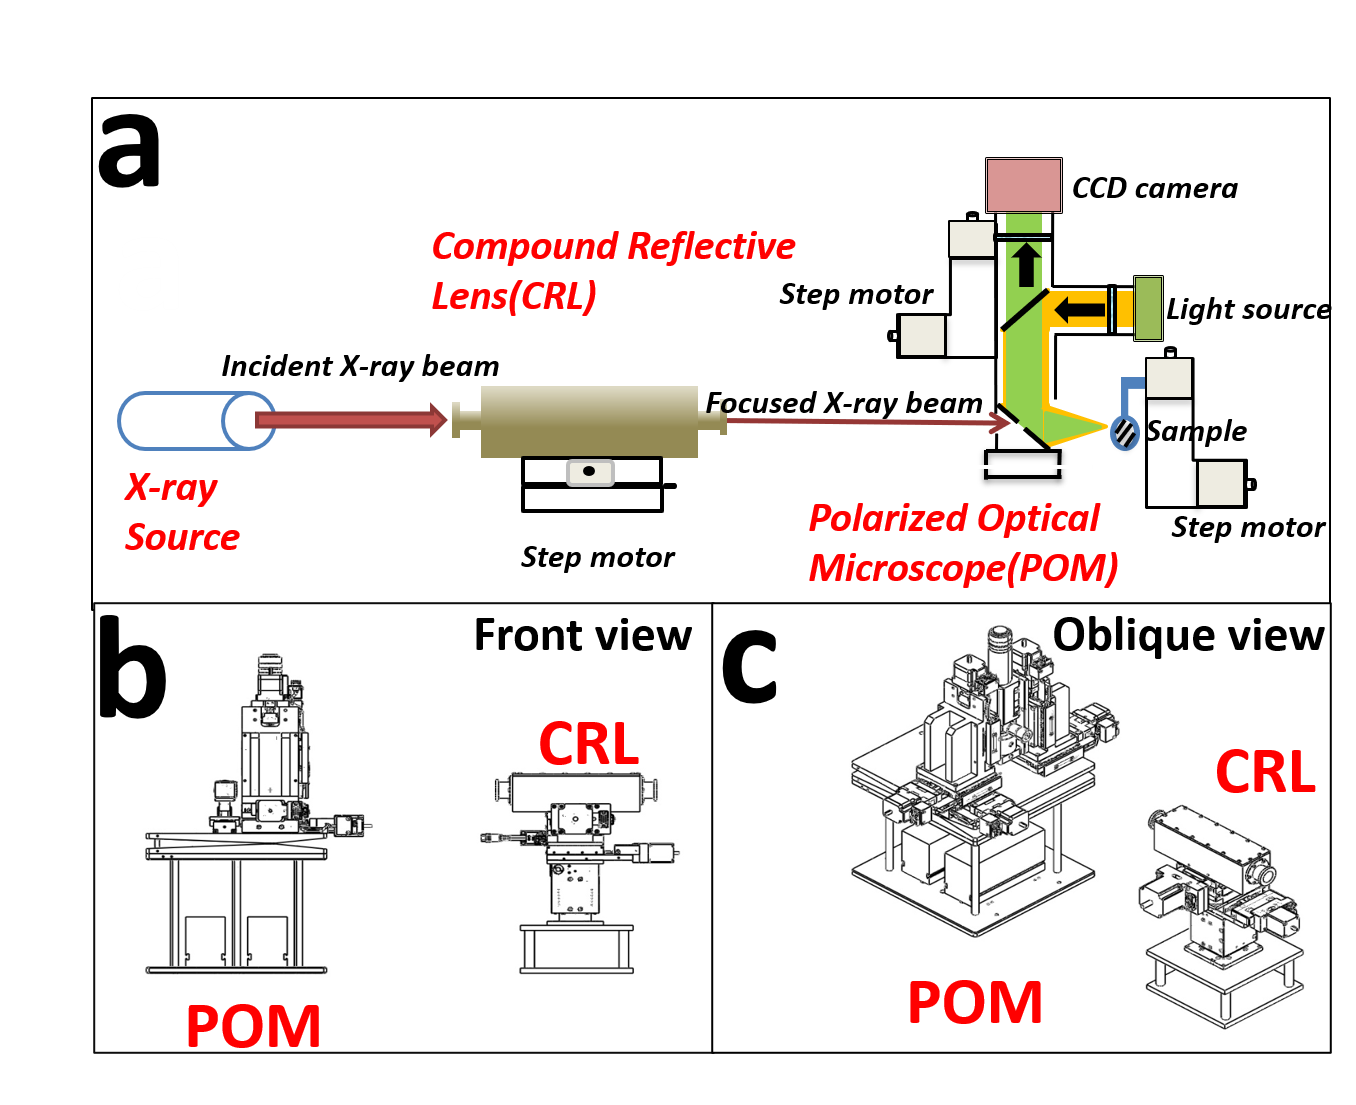
\includegraphics[scale=0.5]{Figures/Fig1WholeSystem.png}
  \caption{Whole system}
  \label{WholeSystem}
\end{figure}


To improve the spatial resolution of synchrotron radiation experiment, the world’s advanced synchrotron radiation light sources all use micro-focusing to focus the spot to the micron or even sub-micron level.
Representative beamline stations include DSEY-PETRA \uppercase\expandafter{\romannumeral3} P03, SSRF BL15U1.
However, limited by the distance between the sample and the detector, SAXS experiment can not be implemented on these stations.


The main components used for X-ray beam focusing are Kirkpatrick-Baez mirror, Fresnel zone plates, Capillary Optical Lens and Compound Refractive Lenses.
In synchrotron radiation area, Kirkpatrick-Baez mirror(K-B mirror) and Compound Refractive Lenses(CRLs) are more widely used.
The advantages of K-B mirror are aberration-free imaging on both horizontal and vertical planes, no dispersion, high energy, high reflectivity and low flux loss.
However, there are some disadvantages which should be considered.
K-B mirror micro-beam focusing needs to be achieved by adjusting the K-B two mirrors and multi-axis spatial attitude, including: the angle at which X-rays are incident on the mirrors, the vertical angle of the two mirrors, spatial parallelism of two vertical cylinders.
The deployment of K-B mirror changes the original optical path.
As a result, this off-axis device increases the complexity of installation of itself and other experimental equipment.
This is unfavorable for the entire micro-focusing experiment process.


\begin{figure}
  \centering
  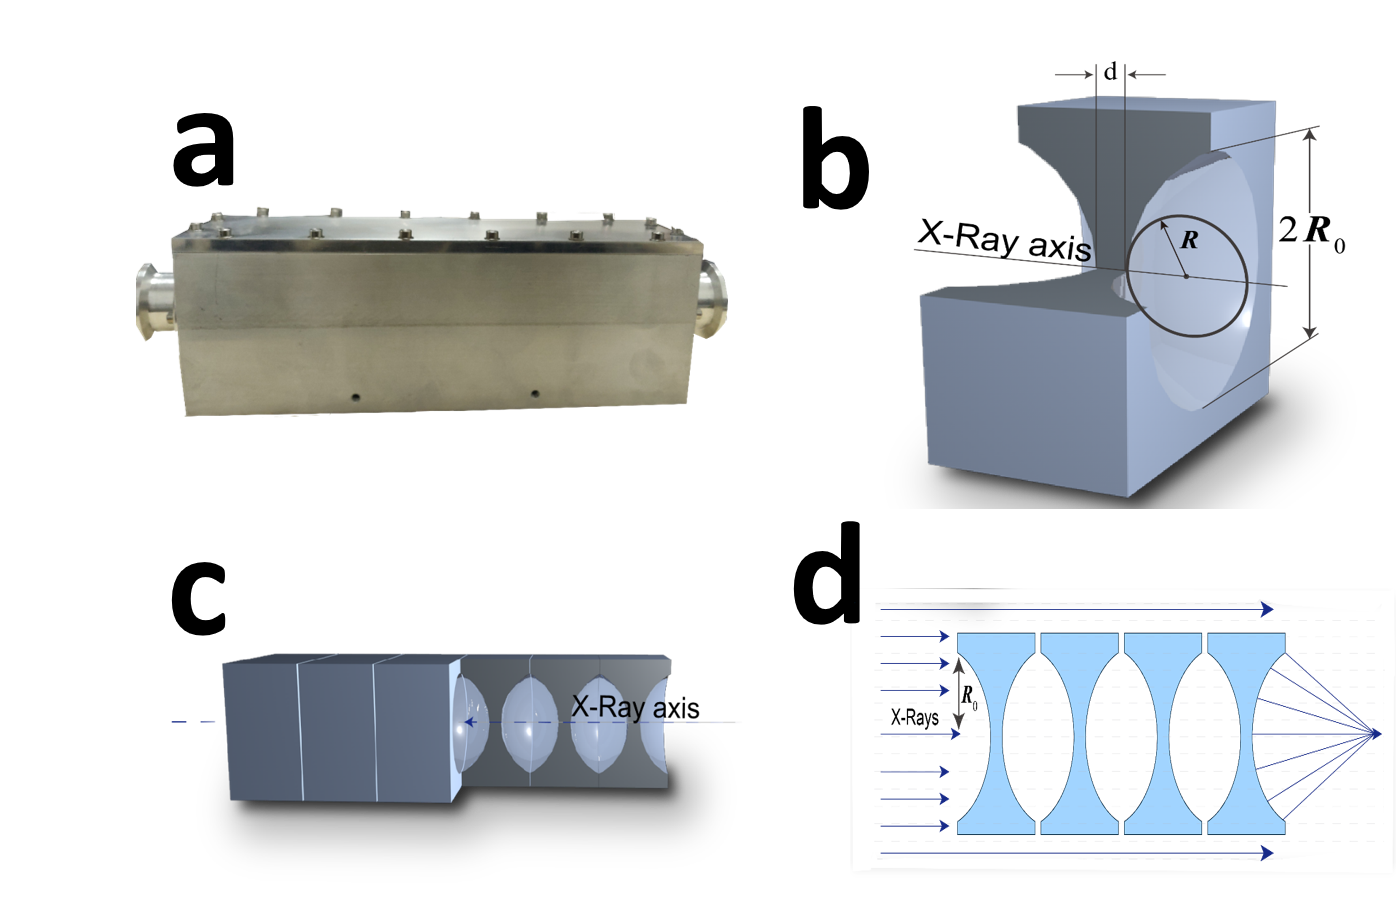
\includegraphics[scale=0.5]{Figures/Fig2CRL.png}
  \caption{Structure of Compound Reflective Lens}
  \label{CRL}
\end{figure}
Compound Refractive Lenses(CRLs) are composed of a series of single lenses arranged in a linear array to achieve X-ray focusing in the energy range of 5-40 keV.
As shown in \autoref{CRL}, the most widely used CRLs are parabolic compound refraction lenses.
The parabolic compound refraction lens has a parabolic surface that rotates around the axis of symmetry to form a parabola.
It can focus X-rays in two dimensions without causing aberrations in theory.
Compared to K-B mirror, CRL does not change the original optical path propagation direction, has good high temperature stability and easy cooling, simple and compact structure, easy to adjust, low requirements for lens surface roughness, relatively insensitive to vibration and many other advantages.
The disadvantage of CRL is the low transmission efficiency.
Because the aperture of the diaphragm is small and the X-rays are absorbed when they penetrate the lens material, the focused light intensity will drop by one to two orders of magnitude.
Despite this, the luminous flux can be maintained at $\mathrm{10^{10}\sim 10^{11} phs/s}$ after using CRL to focus the spot.
This flux is enough to study the structure of crystalline polymers.

\begin{figure}
  \centering
  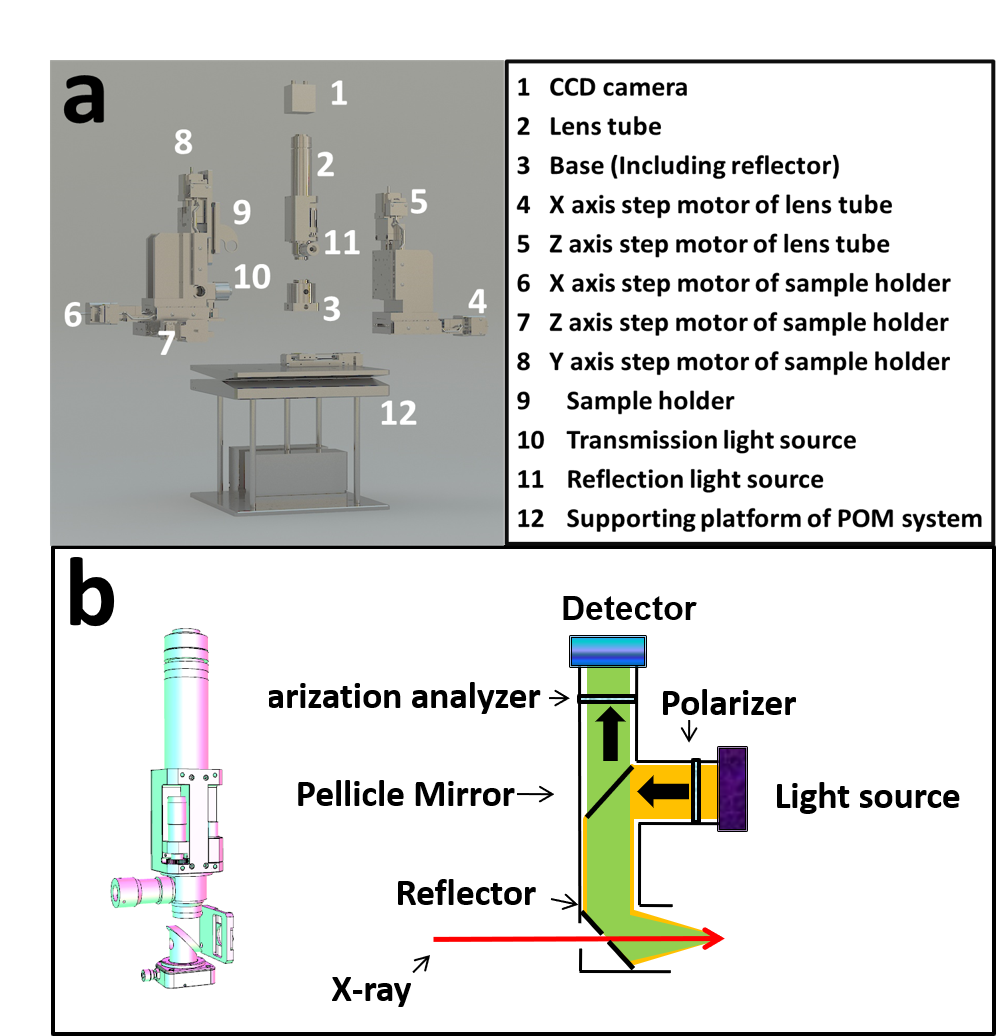
\includegraphics[scale=0.5]{Figures/Fig3POM.png}
  \caption{POM overall disassembly and lens cone disassembly}
  \label{POM}
\end{figure}
Polarized Optical Microscope(POM) is a simple and intuitive method for studying polymer crystal morphology.
\autoref{POM} is a schematic diagram of the disassembly of a POM.
When the polarized light generated by the polarizer and the analyzer enters the anisotropic polymer crystal, birefringence occurs, and the crystal contrast is obtained through the coherence of the polarized light.
Different crystal forms of polymers, such as spherulites, string crystals, stretched chain crystals, transverse crystals, etc., all have anisotropic optical properties, so their crystal morphology, size, number, etc. can be observed with a POM.


In this passage, a combined device of micro-focus synchrotron radiation small-angle scattering and polarizing microscope is proposed.
A series of parameters of the device are adjusted, and the device is used to characterize the crystalline morphology and microstructure of related polymers.
\section{Experiment}
\subsection{CRL parameter determination}
CRL's parameter selection mainly includes its material, type and number of pieces.
The energy of X-ray at BL19U2 is mainly 12 keV.
In this energy, materials with low atomic number have less absorption of X-rays.
For this reason, a beryllium CRL was chosen.


There are three common single lens, is the parameters of them.
Considering the size of the lens container, lens with 50 $\mathrm{\mu m}$ was chosen.
\begin{table}
  \centering
  \caption{Parameters of several common single lens}
  \begin{tabular}{ccc}
    \toprule
    Radius $R$/$\mathrm{\mu m}$ & Aperture 2$R_0$/$\mathrm{\mu m}$ & Area $\pi R_0^2$/$\mathrm{mm^{-2}}$ \\
    \midrule
    200                         & 881                              & 0.609                               \\
    100                         & 623                              & 0.305                               \\
    50                          & 440                              & 0.152                               \\
    \bottomrule
  \end{tabular}
  \label{CRL parameters}
\end{table}

According to the actual situation of beamline station shed size and pipeline layout.
Transmittance refers to the ratio of the light intensity after passing through the lens and the light intensity without passing through the lens.
It can be calculated by \autoref{transmission equation}:
\begin{equation}
  T_p=\frac{\int_0^{2\pi}\mathrm{d}\theta\int_0^{R_0}e^{-\mu ND(r)}r\mathrm{d}r}{\int_0^{2\pi}\mathrm{d}\theta\int_0^{R_0}r\mathrm{d}r}=\frac{1-e^{-a}}{a}e^{-\mu Nd}
  \label{transmission equation}
\end{equation}
In \autoref{transmission equation}, $a=\mu N R_0^2/R$, $R$ and $R_o$ are given in \autoref{CRL parameters}, $N$ is the number of lens; $d$ is the minimum thickness of a single mirror.
For parabolic lenses, d can be calculated with the following equation:
\begin{equation}
  D(r)=d+2\times \frac{r^2}{2R}
  \label{width}
\end{equation}
The maximum processing thickness $D(r)$ of the CRL selected in this experiment is 2 mm.
Substituting $D(r)$ and $r=R_0$ into the \autoref{width}, the minimum d equals 1.032 mm.


According to the actual situation of beamline station shed size and pipeline layout, the image distance is about 400 mm and so is the focal length.
After a series of calculations, 30 is an appropriate number of lenses.
Substituting $N=30$ and $d=1.032$ into the \autoref{transmission equation}, $T_p$ equals 0.327.


The flux of photons after passing through the lens can be calculated by the following equation:
\begin{equation}
  I=i\times T_p \times R
  \label{intensity}
\end{equation}
$i$ is the flux of incident X-ray.
In BL19U2, under 220 mA current intensity, $i=2.5\times 10^{12}$ photons/s, $R$ is the photon acceptance rate and equals 0.0598.
Substituting these values into the \autoref{intensity}, $I$ equals $4.89\times 10^{10}$ photons/s. This value is enough to study the structure of crystalline polymers.
\subsection{Construction of the joint system}
\begin{figure}
  \centering
  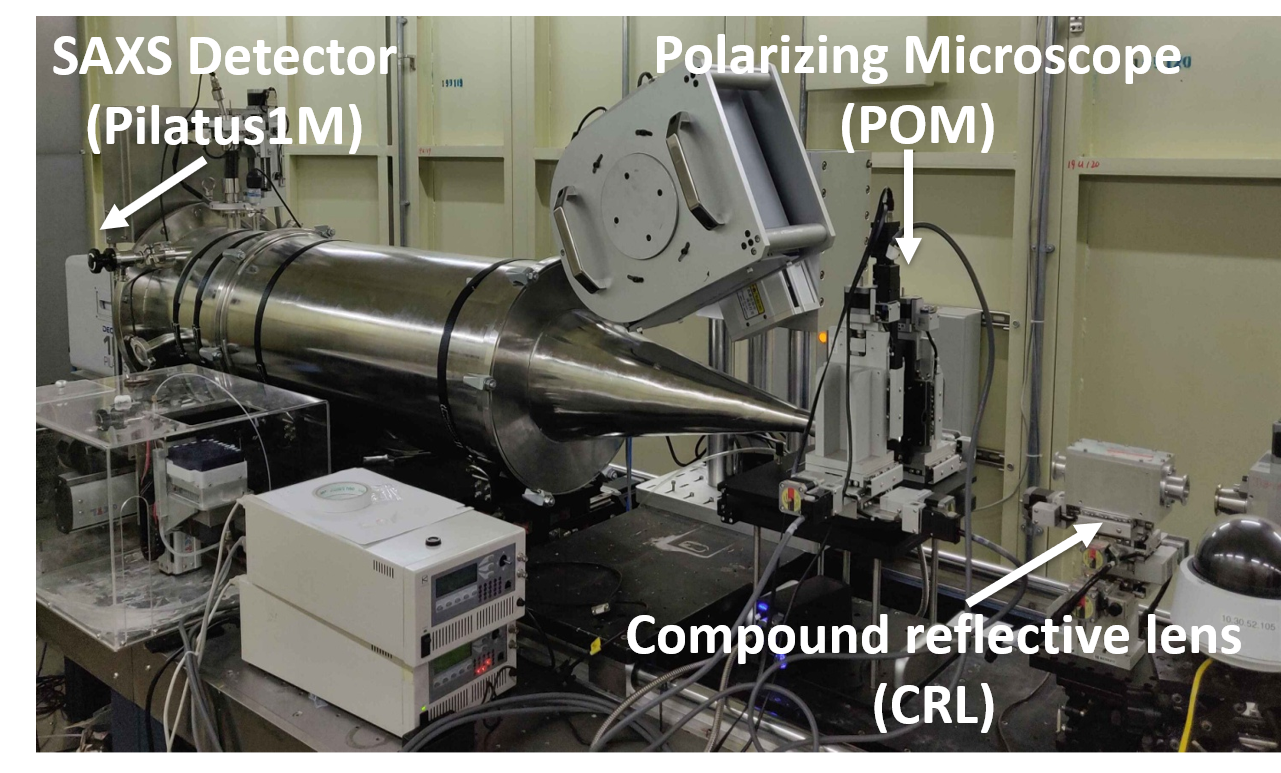
\includegraphics[scale=0.5]{Figures/Fig4SiteMap.png}
  \caption{Site map of the system}
  \label{sitemap}
\end{figure}
\autoref{WholeSystem} is the schematic diagram of the structure of synchrotron radiation X-ray micro-focusing polarized microscopy system.
The combined system includes a micro-focusing component and an in-situ polarized light microscope system.
After the incident X-ray is focused by the CRL, it will pass through the light hole on the lower side of the POM, and then the scattered signal will be received by the detector.
The on-site construction diagram of the system is shown in \autoref{sitemap}.
\section{Application}

\end{document}